\documentclass[border=1pt,tikz]{standalone}
\usepackage{tikzlings}

\newcounter{quack}

\makeatletter
\newcommand{\rhinohookbody}{
  \filldraw[\rhino@mouth,line width=\scalingfactor*0.4pt] (0.125, 1.5) arc [start angle=-50, end angle=-130, radius=0.2] -- cycle;
}
\makeatother

\begin{document}

\foreach \macro in {90,...,61}{
  \setcounter{quack}{\macro}
  \addtocounter{quack}{-10}

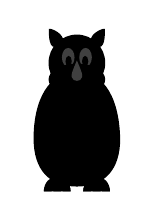
\begin{tikzpicture}
    \rhino[
      body=black!\macro!white,
      eye=darkgray!\macro!white,
      horn=darkgray!\macro!white,
    ]
\end{tikzpicture}
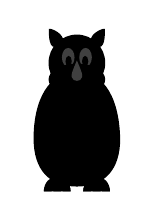
\begin{tikzpicture}
    \rhino[
      body=black!\macro!white,
      eye=darkgray!\macro!white,
      horn=darkgray!\macro!white,
    ]
\end{tikzpicture}
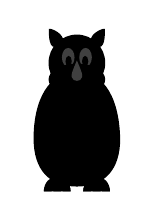
\begin{tikzpicture}
    \rhino[
      body=black!\macro!white,
      eye=darkgray!\macro!white,
      horn=darkgray!\macro!white,
    ]
\end{tikzpicture}
}

\end{document}